\documentclass[12pt]{article}
\usepackage[spanish]{babel}
\usepackage[utf8]{inputenc}
\usepackage{amsmath}
\usepackage{graphicx}
\usepackage{booktabs}
\usepackage{array}
\usepackage{multirow}
\usepackage{float}
\usepackage{longtable}
\usepackage{subcaption}
\usepackage{wrapfig}
\usepackage{tikz}
\usetikzlibrary{arrows.meta, positioning, shapes.geometric}
\title{Proyecto 3: Reemplazo de Equipos}
\author{Emily Sanchez \\ Viviana Vargas \\[1cm] Curso: Investigación de Operaciones \\ II Semestre 2025}
\date{\today}

\begin{document}

\maketitle
\newpage
\section*{Problema de Reemplazo de Equipos}
El algoritmo de reemplazo de equipos se utiliza en Investigación de Operaciones para decidir cuándo conviene reemplazar una máquina o equipo que se deteriora con el tiempo.\\
La idea básica es comparar dos tipos de costos:\\
\begin{itemize}
\item \textbf{Costo de mantener el equipo actual:} Incluye reparaciones, mantenimiento y costos de operación, que normalmente aumentan con los años de uso.\\
\item \textbf{Costo de reemplazarlo por uno nuevo:} Incluye el costo inicial de adquisición y el valor de rescate (lo obtenido al vender el equipo viejo).\\
\end{itemize}
El objetivo es minimizar el costo promedio anual (o el valor presente de los costos) a lo largo del tiempo.\\
\textbf{Variaciones comunes del problema:}\\
\begin{itemize}
\item \textbf{Ganancias por año:} La productividad del equipo disminuye con la edad, afectando los ingresos.\\
\item \textbf{Inflación:} Los precios de adquisición y mantenimiento cambian según el año.\\
\item \textbf{Nuevas tecnologías:} Equipos más modernos pueden ofrecer mejores rendimientos y menores costos operativos.\\
\end{itemize}
\textbf{Fórmula del costo:} $C_{t,j} = \text{Compra} + \sum \text{Mantenimiento}_k - \text{Venta}_{j-t}$\\
\textbf{Algoritmo:} Programación Dinámica \\
\textbf{Función recursiva:} $g(t) = \min\limits_{j=t+1}^{\min(t+\text{vida útil}, n)} \{C_{t,j} + g(j)\}$ con $g(n) = 0$\\

\section*{Datos del Problema}
\begin{itemize}
\item Costo inicial (compra): \$500.00
\item Plazo del proyecto: 3 años
\item Vida útil del equipo: 4 años
\end{itemize}

\begin{table}[H]
\centering
\caption{Datos del equipo por año de uso}
\begin{tabular}{ccc}
\toprule
Año de Uso & Mantenimiento & Valor Residual \\
\midrule
1 & \$30.00 & \$400.00 \\
2 & \$40.00 & \$300.00 \\
3 & \$60.00 & \$250.00 \\
\bottomrule
\end{tabular}
\end{table}

\clearpage
\section*{Cálculo de Costos $C_{t,j}$}
\begin{longtable}{cccc}
\caption{Cálculo detallado de costos por período} \\
\toprule
Período (t-j) & Duración & Fórmula & Costo \\
\midrule
\endfirsthead
\multicolumn{4}{c}{\tablename\ \thetable\ -- Continúa} \\
\toprule
Período (t-j) & Duración & Fórmula & Costo \\
\midrule
\endhead
\midrule
\multicolumn{4}{r}{Continúa en la siguiente página} \\
\endfoot
\bottomrule
\endlastfoot
0-1 & 1 año & $500 + 30 - 400$ & \$130.00 \\
0-2 & 2 años & $500 + 30 + 40 - 300$ & \$270.00 \\
0-3 & 3 años & $500 + 30 + 40 + 60 - 250$ & \$380.00 \\
1-2 & 1 año & $500 + 30 - 400$ & \$130.00 \\
1-3 & 2 años & $500 + 30 + 40 - 300$ & \$270.00 \\
2-3 & 1 año & $500 + 30 - 400$ & \$130.00 \\
\end{longtable}

\clearpage
\section*{Cálculo de $g(t)$ (Programación Dinámica)}
\begin{itemize}
\item $g(3) = 0$ (caso base)
\item $g(2) = \min\{ \mathbf{C_{2,3} + g(3) = 130.00}\} = \$130.00$ \textbf{(j=3)}
\item $g(1) = \min\{ \mathbf{C_{1,2} + g(2) = 260.00}, C_{1,3} + g(3) = 270.00\} = \$260.00$ \textbf{(j=2)}
\item $g(0) = \min\{ C_{0,1} + g(1) = 390.00, C_{0,2} + g(2) = 400.00, \mathbf{C_{0,3} + g(3) = 380.00}\} = \$380.00$ \textbf{(j=3)}
\end{itemize}

\subsection*{Empates}
Se han resaltado en \textbf{negrita} las opciones óptimas.\\
\textbf{No se encontraron empates.} Existe una única estrategia óptima para cada año de inicio.\\
\clearpage
\section*{Solución Óptima}
\textbf{Costo mínimo total:} \$380.00\\
\textbf{Planes óptimos encontrados:} 1
\subsection*{Grafos de Planes Óptimos}
A continuación se presentan los grafos de \emph{saltos de rana} para cada plan óptimo encontrado.

\begin{figure}[H]
\centering
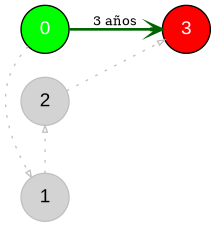
\includegraphics[width=0.8\textwidth]{Reemplazo_Bici_plan_1.png}
\caption{Plan Óptimo 1: \texttt{0-3}}
\label{fig:plan1}
\end{figure}

\textbf{Plan 1:} \texttt{0-3}
\begin{itemize}\small
\item Período 0-3: 3 años, Costo: \$380.00
\end{itemize}

\end{document}
